%%%%%%%%%%%%%%%%%%%%%%%%%%%%%%%%%%%%%%%%%
% Dreuw & Deselaer's Poster
% LaTeX Template
% Version 1.0 (11/04/13)
%
% Created by:
% Philippe Dreuw and Thomas Deselaers
% http://www-i6.informatik.rwth-aachen.de/~dreuw/latexbeamerposter.php
%
% This template has been downloaded from:
% http://www.LaTeXTemplates.com
%
% License:
% CC BY-NC-SA 3.0 (http://creativecommons.org/licenses/by-nc-sa/3.0/)
%
%%%%%%%%%%%%%%%%%%%%%%%%%%%%%%%%%%%%%%%%%

%----------------------------------------------------------------------------------------
%	PACKAGES AND OTHER DOCUMENT CONFIGURATIONS
%----------------------------------------------------------------------------------------

\documentclass[final,hyperref={pdfpagelabels=false}]{beamer}

\usepackage[orientation=portrait,size=a0,scale=1.4]{beamerposter} % Use the beamerposter package for laying out the poster with a portrait orientation and an a0 paper size

\usepackage[utf8]{inputenc} % Enable åäö

\usetheme{I6pd2} % Use the I6pd2 theme supplied with this template

\usepackage[english]{babel} % English language/hyphenation

\usepackage{amsmath,amsthm,amssymb,latexsym} % For including math equations, theorems, symbols, etc

%\usepackage{times}\usefonttheme{professionalfonts}  % Uncomment to use Times as the main font
\usefonttheme[onlymath]{serif} % Uncomment to use a Serif font within math environments

\boldmath % Use bold for everything within the math environment

\usepackage{booktabs} % Top and bottom rules for tables

\graphicspath{{figures/}} % Location of the graphics files

\usecaptiontemplate{\small\structure{\insertcaptionname~\insertcaptionnumber: }\insertcaption} % A fix for figure numbering

%----------------------------------------------------------------------------------------
%	TITLE SECTION 
%----------------------------------------------------------------------------------------

\title{\huge Kitchen Occupation} % Poster title

\author{People counting using depth sensors.} % Author(s)

\institute{Department of Electrical Engineering, Linköping University} % Institution(s)

%----------------------------------------------------------------------------------------
%	FOOTER TEXT
%----------------------------------------------------------------------------------------

\newcommand{\leftfoot}{Created by: Erik Fall, Gustav Häger, Malin Rudin, Alexander Sjöholm, Martin Svensson, Mattias Tiger and Nikolaus West} % Left footer text

\newcommand{\rightfoot}{} %{http://www.densekitchen.bloip.se} % Right footer text

%----------------------------------------------------------------------------------------

\begin{document}

\addtobeamertemplate{block end}{}{\vspace*{2ex}} % White space under blocks

\begin{frame}[t] % The whole poster is enclosed in one beamer frame

\begin{columns}[t] % The whole poster consists of two major columns, each of which can be subdivided further with another \begin{columns} block - the [t] argument aligns each column's content to the top

\begin{column}{.02\textwidth}\end{column} % Empty spacer column

\begin{column}{.465\textwidth} % The first column

%----------------------------------------------------------------------------------------
%	OBJECTIVES
%----------------------------------------------------------------------------------------

\begin{block}{Objectives}

\begin{enumerate}
\item Create a system to monitor room usage intensity, primarily focusing on student kitchens.
\item The system needs to be cheap and easy to install and maintain.
\item The system should provide real-time information about room usage intensity.
\end{enumerate}

\end{block}

%----------------------------------------------------------------------------------------
%	Hardware setup
%----------------------------------------------------------------------------------------

\begin{block}{System}

\begin{columns} % Subdivide the first main column
\begin{column}{.54\textwidth} % The first subdivided column within the first main column
\begin{itemize}
\item Hardware setup.
\begin{itemize}
\item Stuff about the setup.
\end{itemize}
\item Portability.
\begin{itemize}
\item Stuff about supported sensors and platforms.
\end{itemize}
\end{itemize}
\end{column}

\begin{column}{.43\textwidth} % The second subdivided column within the first main column
\centering
\begin{figure}

\includegraphics[width=0.8\linewidth]{placeholder.jpg}
\caption{Figure caption}
\end{figure}
\end{column}
\end{columns} % End of the subdivision

\begin{itemize}
\item Performance requirements.
\begin{itemize}
\item Herpa derpa derpa.
\item derp herrrp derp.
\item Walla.
\end{itemize}
\end{itemize}

\end{block}

%----------------------------------------------------------------------------------------
%	Software system
%----------------------------------------------------------------------------------------

\begin{block}{Software}

\begin{itemize}
\item The software pipeline
\begin{itemize}
\item Suspendisse potenti. Fusce a est eget turpis rhoncus varius sed sed dui. Cras justo nibh, bibendum a cursus eget, consequat et dui. Maecenas vel nisl elit, sed dignissim dolor. 
\item In hac habitasse platea dictumst.
\end{itemize}

\item The GUIs
\begin{itemize}
\item Cum sociis natoque penatibus et magnis dis parturient montes, nascetur ridiculus mus. 
\item Proin in nisi diam.
\item Nam ultricies pellentesque nunc, ultrices volutpat nisl ultrices a.
\end{itemize}

\item Configuration 
\begin{itemize}
\item Duis semper lorem eget dui dignissim porttitor.
\item Nulla facilisi. In ullamcorper lorem quis dolor.
\end{itemize}
\end{itemize}

\end{block}

%----------------------------------------------------------------------------------------
%	User Interface
%----------------------------------------------------------------------------------------

\begin{block}{Dense Debugger}

\begin{columns} % Subdivide the first main column
\begin{column}{.54\textwidth} % The first subdivided column within the first main column

\begin{itemize}
\item Transparent and flexible pipeline overview.
\item Online low-level profiling for every module.
\item Configuration interface

\begin{itemize}
\item Doors (green)
\item Entering checkpoints (circles)
\item Exclusions (red)
\end{itemize}
\end{itemize}

\end{column}

\begin{column}{.43\textwidth} % The second subdivided column within the first main column
\centering
\begin{figure}
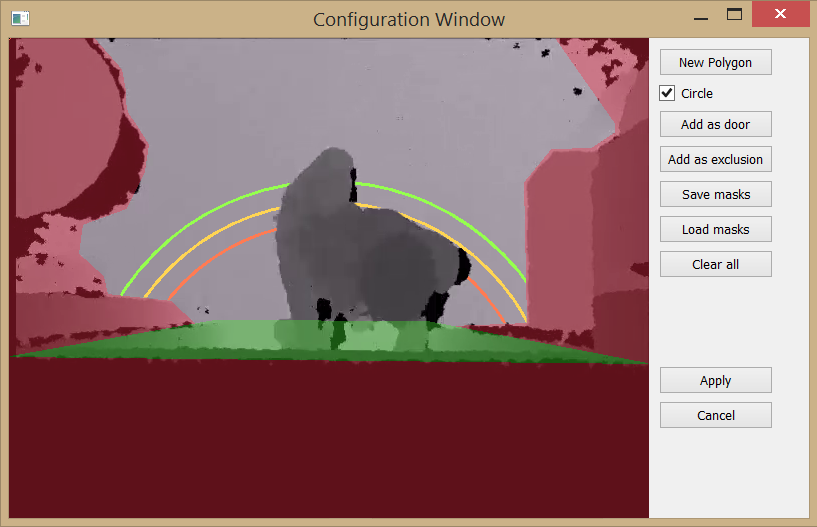
\includegraphics[width=\linewidth]{PosterConfig.png}
\label{fig:Config}
\caption{Visualization of configurables}
\end{figure}
\end{column}
\end{columns} % End of the subdivision

\begin{figure}
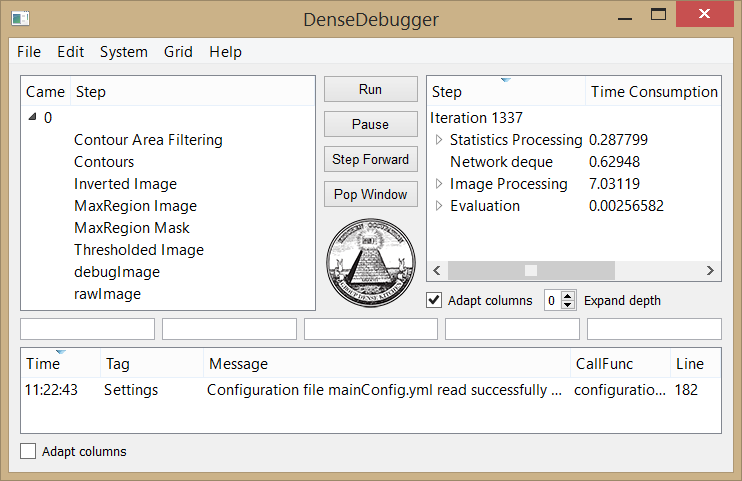
\includegraphics[width=\linewidth]{PosterDebugger.png}
\caption{}
\end{figure}

\end{block}

% ----- NEW COLUMN ---------------------------------------------

\end{column} % End of the first column

\begin{column}{.03\textwidth}\end{column} % Empty spacer column
 
\begin{column}{.465\textwidth} % The second column

% ----- NEW COLUMN ---------------------------------------------

%----------------------------------------------------------------------------------------
%	Pepole counting
%----------------------------------------------------------------------------------------

\begin{block}{Image Processing}

\begin{itemize}
\item Human segmentation.
\begin{itemize}
\item The human segmentation is based on the assumption that human heads are distinguishable modes in the depth image and that people moving very close to each other seldom differ much more than a head in height. The later assumption seem to hold more often than one might think, as supported by over 5 hours of test data. The segmentation is realized by a series of threshold and morphological operations, gaussian blurring, contour drawing and searches for local maxima's. 
\end{itemize}
\item Tracking and counting.
\begin{itemize}
\item{The tracker pairs objects with each other from previous frame to the next. Pairs closest matching objects. Handles occlution, outliers and noise.}
\item{Counting is done using user specified checkpoint lines and a door area.}
\end{itemize}
\item Queue detection.
\begin{itemize}
\item{detecting queues}
\end{itemize}
\end{itemize}

\end{block}

%----------------------------------------------------------------------------------------



%----------------------------------------------------------------------------------------
%	RESULTS
%----------------------------------------------------------------------------------------


\begin{block}{Results: Table}

\begin{itemize}
\item Final system performance
\end{itemize}

\begin{equation}
\label{eq:in_accuracy}
A_{in} = 1 - |\frac{\sum_{frames}{in_{Est}}-\sum_{frames}{in_{GT}}}{\sum_{frames}in_{GT}}|
\end{equation} 

\begin{equation}
\label{eq:out_accuracy}
A_{out} = 1 - |\frac{\sum_{frames}{out_{Est}}-\sum_{frames}out_{GT}}{\sum_{frames}out_{GT}}| 
\end{equation} 


\begin{table}[h]
\centering
	\begin{tabular}{r | c | c | c | c | c | c }
		\emph{Sequence Name}		&  Total entered (GT) & \emph{$A_{in}$} & Total exited (GT) & \emph{$A_{out}$} \\
		\hline \hline
		Data seq. 1			& 108 (108) people & 99 \% & 101 (104) people & 97 \% \\
		Data seq. 2			& 122 (141) people & 87 \% & 77 (91) people & 85 \%  \\
		\end{tabular}
	\caption{System performance in the two evaluation sequences}
\end{table}

\begin{itemize}
\item Data seq. 1 \& Data seq. 2 are two data sequences of 30 minutes each. 
\end{itemize}
     
\end{block}

%------------------------------------------------

\begin{block}{Results: Figure}

\begin{figure}

\includegraphics[width=0.8\linewidth]{placeholder.jpg}
\caption{Resulting accuracy}
\end{figure}

\end{block}

%----------------------------------------------------------------------------------------
%	CONCLUSION
%----------------------------------------------------------------------------------------

\begin{block}{Conclusion}

\begin{itemize}
\item The system provides high-precision people counting using the Microsoft Kinect sensors.
\item The software architecture enables fast implementing and testing of different algorithms.
\item SOMETHING MORE
\end{itemize}

\end{block}

%----------------------------------------------------------------------------------------
%	REFERENCES
%----------------------------------------------------------------------------------------
%
%\begin{block}{References ??}
%        
%\nocite{*} % Insert publications even if they are not cited in the poster
%\small{\bibliographystyle{unsrt}
%\bibliography{sample}}
%
%\end{block}
%
%%----------------------------------------------------------------------------------------
%%	ACKNOWLEDGEMENTS
%%----------------------------------------------------------------------------------------
%
%\begin{block}{Acknowledgments ?? }
%
%\begin{itemize}
%\item We would like to thank the members of Computer Vision Laboratory here at the university for their endless support and for beign able to provide new sensors and hardware with short notice.
%\end{itemize}
%
%\end{block}

%----------------------------------------------------------------------------------------
%	CONTACT INFORMATION
%----------------------------------------------------------------------------------------

%\setbeamercolor{block title}{fg=black,bg=orange!70} % Change the block title color
%
%\begin{block}{Contact Information}
%
%\begin{itemize}
%\item Web: \href{http://www.university.edu/smithlab}{http://www.university.edu/smithlab}
%\item Email: \href{mailto:john@smith.com}{john@smith.com}
%\item Phone: +1 (000) 111 1111
%\end{itemize}
%
%\end{block}

%----------------------------------------------------------------------------------------

\end{column} % End of the second column

\begin{column}{.015\textwidth}\end{column} % Empty spacer column

\end{columns} % End of all the columns in the poster

\end{frame} % End of the enclosing frame

\end{document}